% THIS IS SIGPROC-SP.TEX - VERSION 3.1
% WORKS WITH V3.2SP OF ACM_PROC_ARTICLE-SP.CLS
% APRIL 2009
%
% It is an example file showing how to use the 'acm_proc_article-sp.cls' V3.2SP
% LaTeX2e document class file for Conference Proceedings submissions.
% ----------------------------------------------------------------------------------------------------------------
% This .tex file (and associated .cls V3.2SP) *DOES NOT* produce:
%       1) The Permission Statement
%       2) The Conference (location) Info information
%       3) The Copyright Line with ACM data
%       4) Page numbering
% ---------------------------------------------------------------------------------------------------------------
% It is an example which *does* use the .bib file (from which the .bbl file
% is produced).
% REMEMBER HOWEVER: After having produced the .bbl file,
% and prior to final submission,
% you need to 'insert'  your .bbl file into your source .tex file so as to provide
% ONE 'self-contained' source file.
%
% Questions regarding SIGS should be sent to
% Adrienne Griscti ---> griscti@acm.org
%
% Questions/suggestions regarding the guidelines, .tex and .cls files, etc. to
% Gerald Murray ---> murray@hq.acm.org
%
% For tracking purposes - this is V3.1SP - APRIL 2009

\documentclass{acm_proc_article-sp}
\graphicspath{ {./images/} }
\usepackage{subcaption}

\begin{document}

\title{Forecasting building occupancy: A comparative study of approaches}
%\subtitle{[Extended Abstract]
%\titlenote{A full version of this paper is available as
%\textit{Author's Guide to Preparing ACM SIG Proceedings Using
%\LaTeX$2_\epsilon$\ and BibTeX} at
%\texttt{www.acm.org/eaddress.htm}}}
%
% You need the command \numberofauthors to handle the 'placement
% and alignment' of the authors beneath the title.
%
% For aesthetic reasons, we recommend 'three authors at a time'
% i.e. three 'name/affiliation blocks' be placed beneath the title.
%
% NOTE: You are NOT restricted in how many 'rows' of
% "name/affiliations" may appear. We just ask that you restrict
% the number of 'columns' to three.
%
% Because of the available 'opening page real-estate'
% we ask you to refrain from putting more than six authors
% (two rows with three columns) beneath the article title.
% More than six makes the first-page appear very cluttered indeed.
%
% Use the \alignauthor commands to handle the names
% and affiliations for an 'aesthetic maximum' of six authors.
% Add names, affiliations, addresses for
% the seventh etc. author(s) as the argument for the
% \additionalauthors command.
% These 'additional authors' will be output/set for you
% without further effort on your part as the last section in
% the body of your article BEFORE References or any Appendices.

\numberofauthors{2} %  in this sample file, there are a *total*
% of EIGHT authors. SIX appear on the 'first-page' (for formatting
% reasons) and the remaining two appear in the \additionalauthors section.
%
\author{
% You can go ahead and credit any number of authors here,
% e.g. one 'row of three' or two rows (consisting of one row of three
% and a second row of one, two or three).
%
% The command \alignauthor (no curly braces needed) should
% precede each author name, affiliation/snail-mail address and
% e-mail address. Additionally, tag each line of
% affiliation/address with \affaddr, and tag the
% e-mail address with \email.
%
% 1st. author
\alignauthor
James Howard\\\
       \affaddr{Colorado School of Mines}\\
       \affaddr{1500 Illinois St.}\\
       \affaddr{Golden, CO 80401}\\
       \email{jahoward@mines.edu}
% 2nd. author
\alignauthor
William Hoff\\\
       \affaddr{Colorado School of Mines}\\
       \affaddr{1500 Illinois St.}\\
       \affaddr{Golden, CO 80401}\\
       \email{whoff@mines.edu}
}

\date{17 May 2013}


\maketitle
\begin{abstract}
This paper provides a sample of a \LaTeX\ document which conforms to
the formatting guidelines for ACM SIG Proceedings.
It complements the document \textit{Author's Guide to Preparing
ACM SIG Proceedings Using \LaTeX$2_\epsilon$\ and Bib\TeX}. This
source file has been written with the intention of being
compiled under \LaTeX$2_\epsilon$\ and BibTeX.

The developers have tried to include every imaginable sort
of ``bells and whistles", such as a subtitle, footnotes on
title, subtitle and authors, as well as in the text, and
every optional component (e.g. Acknowledgments, Additional
Authors, Appendices), not to mention examples of
equations, theorems, tables and figures.

To make best use of this sample document, run it through \LaTeX\
and BibTeX, and compare this source code with the printed
output produced by the dvi file.
\end{abstract}

% A category with the (minimum) three required fields
%\category{H.4}{Information Systems Applications}{Miscellaneous}
%A category including the fourth, optional field follows...
%\category{D.2.8}{Software Engineering}{Metrics}[complexity measures, performance measures]

%\terms{Theory}

%\keywords{ACM proceedings, \LaTeX, text tagging} % NOT required for Proceedings

\section{Introduction}

According to the U.S. Department of Energy energy for heating and cooling accounts for approximately 35 - 45\% \cite{DOE2010} of the total expenditure within a building. With such a large investment of energy being used to regulate the temperature of a building, any possible areas of improvement in this area are heavily sought after.   Knowledge of occupancy of people within a building are an important component to intelligent heating and air condition systems.  True levels of occupancy are rarely known and as a results most buildings instead rely on existing systems such as carbon dioxide sensors or motion activated lights.  

A number of other researchers have created local wireless network occupancy sensing devices using a combination of sensors.  In this paper we explore the forecasting accuracy of multiple common time series forecasting models using a number of forecasting measurement metrics.  Or occupancy is derived from infrared sensors densely placed around a building.  The data is collected from two different types of buildings, one is an office building, the other a classroom and research building with different schedules of levels occupancy.  We believe that this work will lead researchers to have a better idea of what forecasting algorithms will perform best under the specific conditions of our buildings.  

The remainder of the paper is laid out as follows: Section 2 discusses the other work in this area including research from vehicle traffic systems.  Section 3 discusses our forecasting models.  In section 4 we introduce the datasets and give a brief description of the data collection method and the types of buildings from which the data was generated.  Section 5 show the results of our forecasts and the paper concludes with a discussion of our conclusions and future work in section 6.

\section{Related work}
There has been considerable work in generating simulated models of occupancy \cite{PAGE2008, GOLDSTEIN2010}.  These simulations often involve agent based models where the concern is more with the accuracy of the models occupancy at any given time instead of the model's forecasting abilities.   Agent based models also tend not to scale well to large buildings where the where large numbers of agents, rooms and interactions lead to non-trivial solutions.

Researchers have also created systems to attempt direct occupancy estimation using a combination of simple sensors and wireless motes.  Agarwal, et. al \cite{Agarwal2010} has created motes using a combination of an IR sensors reed switch place on a door to determine the likelihood that a room is occupied.  This work is excellent for occupancy data acquisition, but little work was done on occupancy forecasting.  Mamidi \cite{Mamidi2012} and the University of Southern California have developed a building-level energy management system using a combination of motion detectors and environmental sensors.  They compared their readings against a ground truth recorded by occupants using specifically monitored rooms.  They used a variety of standard learning algorithms, including ensemble methods to accurately estimate the occupancy of a room.  Work from both those these groups however seems to be more focused on occupancy estimation instead of forecasting.

\begin{figure*}[t!]
\centering
\begin{subfigure}{.4\textwidth}
  \centering
  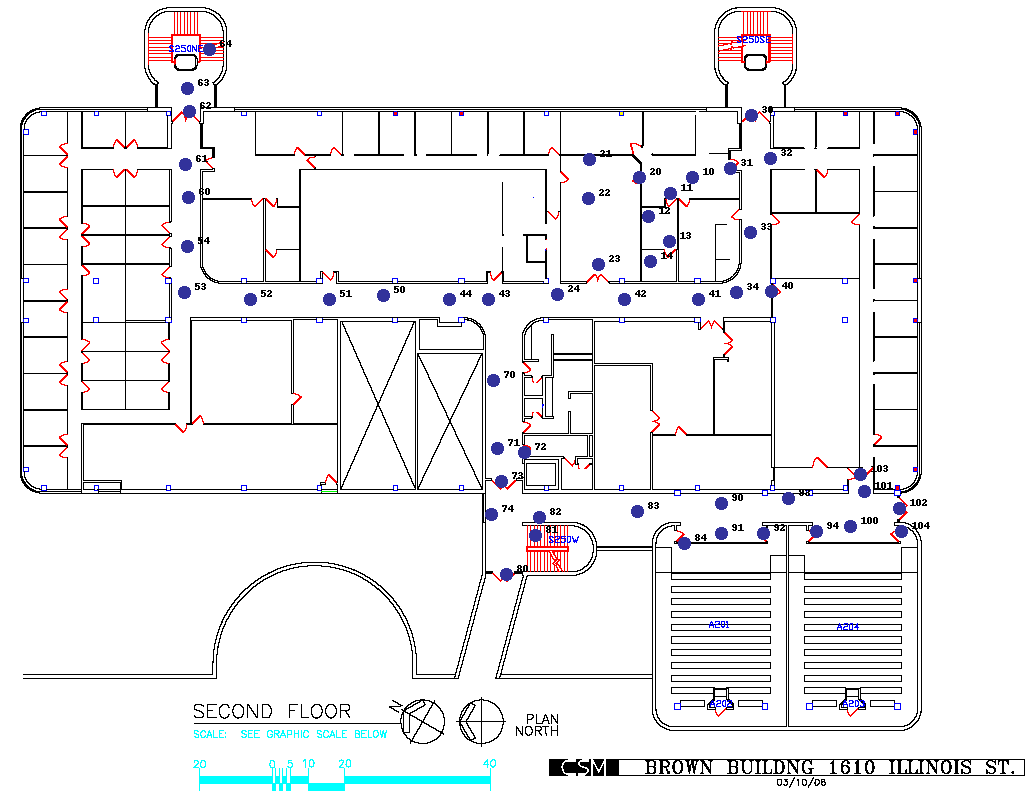
\includegraphics[width=.5\linewidth]{bb_floor2_sensors_old.png}
  \caption{Colorado School of Mines Brown building second floor}
  \label{fig:sub1}
\end{subfigure}
\begin{subfigure}{.4\textwidth}
  \centering
  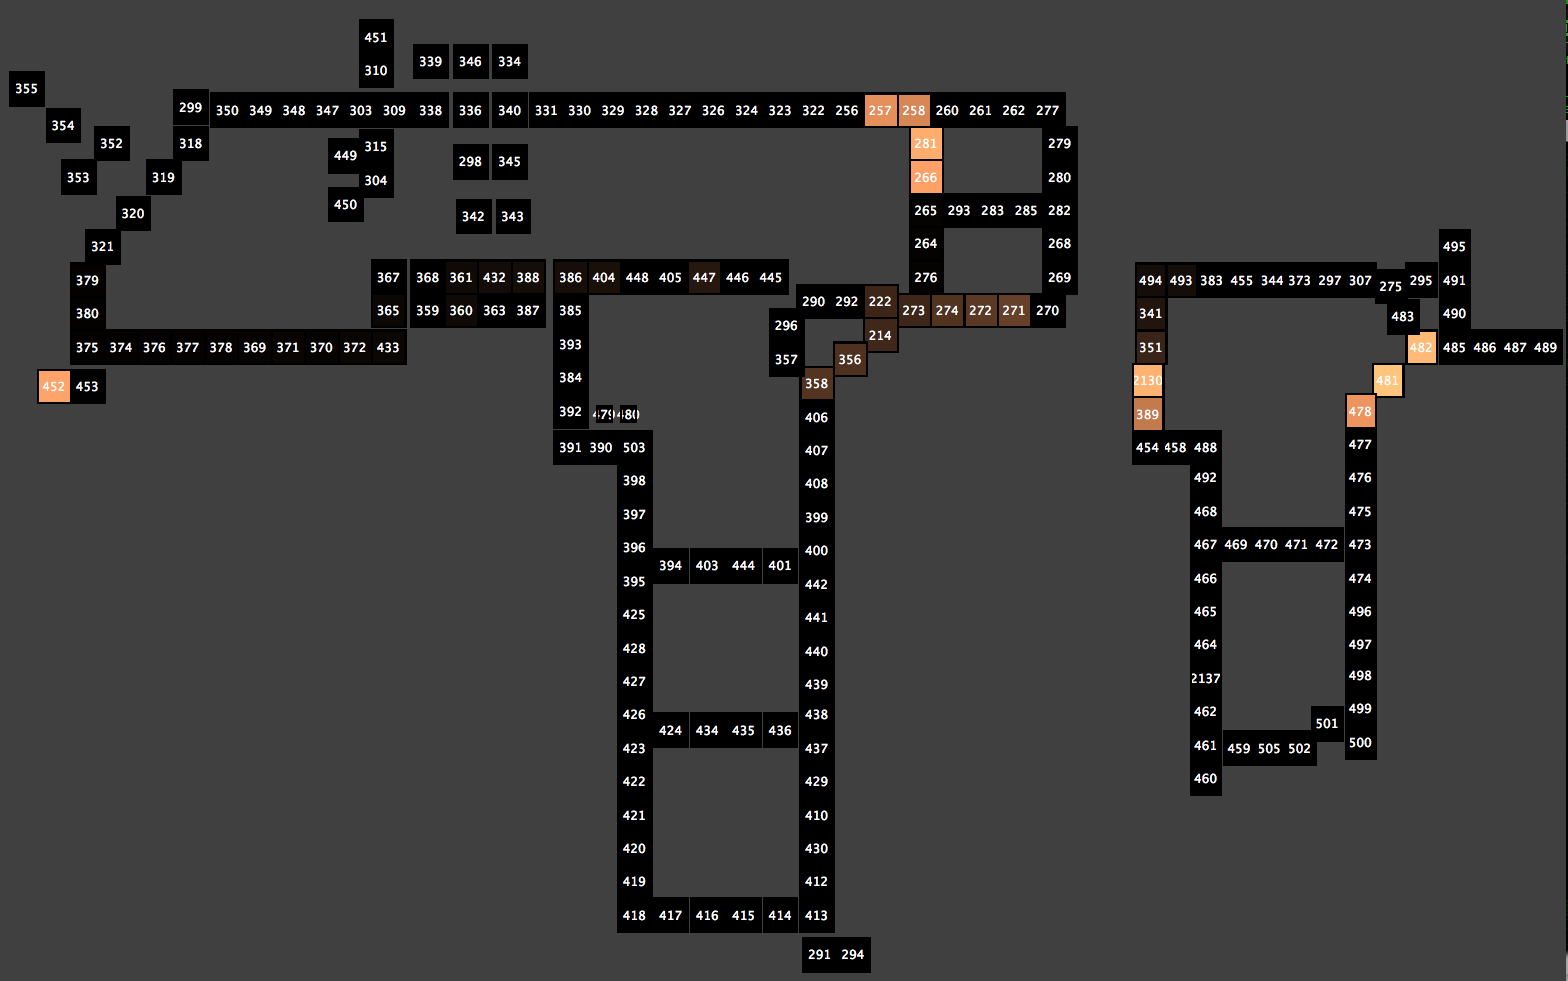
\includegraphics[width=.5\linewidth]{merl_map.png}
  \caption{Merl research lab 7th and 8th floor}
  \label{fig:sub2}
\end{subfigure}
\caption{Sensor locations for buildings}
\label{fig:test}
\end{figure*}


Outside the world of building occupancy forecasting, there has been considerable work with counting vehicles on road ways.  Forecasting for traffic roadways present many of the same challenges that buildings present.  The data has clear daily trends and is subject to large shifts in those trends based on environmental factors such as accidents or weather.  Thus it seems pertinent to discuss any promising forecasting techniques used in the traffic domain along with the building domain.

The classic time series Auto Regressive Moving Average Model (ARMA) or derivations on its form (ARIMA, SARIMA, VARMA, etc) have been used in numerous papers on forecasting.  The results on this class of models seem mixed.  William's \cite{Williams2003} showed promising short term forecasting results using Seasonal ARIMA models on traffic sets from London and Atlanta.  Hong \cite{Hong2011} , while again demonstrating the feasibility of Seasonal ARIMA models to traffic forecasting, achieved better results combining genetic algorithms and simulated annealing.  

Zheng \cite{Zheng2006} used a bayesian combination of time delayed neural networks to achieve better forecasting accuracy than each neural network alone.  This demonstrates the feasibility of both a bayesian combined approach and the use of time delayed neural networks for traffic forecasting.  The problem with these forecasting approaches is that they focus only on short term forecasts, typically one time step into the future (often 15 minutes).  While this forecast horizon may be applicable to traffic forecasting, pre-heating and cooling systems can utilized occupancy forecast up to 24 hours into the future \cite{Ma2010}.  

\section{Occupancy Data}

Our datasets come from two sources.  The first is Mitsubishi's MERL dataset \cite{Wren2007}.  Data is collected here from a collection of roughly 150 passive infrared sensors place densly throughout the 7th and 8th floor of a research building.  The sensors sensors are place roughly two meters apart on the ceilings creating a dense sensing area with little non-sensed space.  Readings are taken at the milisecond level, but due to the sensors settling times the interdetection time of motion is roughly 1.5 seconds.  The data was collected for years and there are roughly 53 million sensor readings.  This building similar to most office buildings with a number of personal offices along with labs and conference rooms.  Employees have roughly set schedules and holdiays are observed as normal.

\begin{figure}[h]
\centering
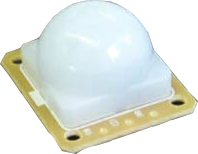
\includegraphics[width = .4\linewidth]{pir_sensor.png}
\caption{Passive infrared motion detector}
\end{figure}

The second dataset is from the Colorado School of Mines (CITE) Brown building.  Data is collected from 50 passive IR sensors mounted on the ceiling of the second floor.  The density of the sensor placement depends on the location within the building.  Outside auditorium is a dense collection of sensors place every meter.  Throughout the rest of the building the sensors are placed roughly every 5 meters.  Data was collected for one academic school year 2008 to 2009 with readings at the one second resolution.  This building operates much differently than the MERL dataset as classes provide motion on a rigid schedule during the day.  Also as students have exams and projects, late night motion is sporadic based on the time of year.    


\section{Forecasting models}
For comparison we select from some of the most common models used for time series forecasting.  This section gives a brief introduction to each of these forecasting models. 

To introduce some notation the data used for these models comes from a set of $M$ binary infrared sensors.  Each of these sensors may sense a person's motion at some time t.  This leaves us with a dataset of the form $\{d^{(s)}_{a}\}$ with $s$ in the set of all sensors $S$ and $a$ is the time of the sensor activation over some time span $A_{span}$.

This data is this aggregated into blocks of 10 minute intervals.  Each block is the sum of all sensor activation for its unit of time.  This leaves us with a dataset of the form $\{y^{(s)}_{t}\}$ where the total number of blocks of time are $T$.

\subsection{Seasonal ARIMA Model}
The Auto Regressive Moving Average Model (ARMA) or derivations on its form (ARIMA, SARIMA, VARMA, etc) have been used in numerous papers on forecasting with applications ranging from economics to vehicle traffic systems \cite{Williams2003, Hong2011}.  

An ARMA model of with a number of $\phi$ and $\theta$ parameters, represented by p and q respectively is defined as: 
\begin{equation}
y_{t} = \phi_{1}y_{t-1} + \phi_{2}y_{t-2} + ... + \phi_{p}y_{t-p} + e_{t} - \theta_{1}e_{t-1} - \theta_{2}e_{t-2} - ... - \theta_{q}e_{t-q}
\end{equation}

\noindent
where $\{y_{t}\}$ denotes the observed time series and $\{e_t\}$ represents an unobserved white noise series.  We abbreviate the model name to ARMA(p, q).  This approach involves training a set of parameters to fit a regression model based on a fixed number of historic readings.  ARMA based approaches are useful for their capability to predict further than one measured time instance in the future.  

Due to our traffic data having periodic trends and a non stationary mean, it is advantageous to use a seasonal ARIMA model.  An ARIMA model can handle non stationary means while periodic trends are handled by the seasonal component of the model.  The seasonal ARIMA model is defined as:
\begin{equation}
\label{eq:sarima}
\phi_{p}(B)\Phi_{p}(B^{season})\nabla^{d}\nabla^{D}_{s}y_{t} = \theta_{q}(B)\Theta_{Q}(B^{season})e_{t}
\end{equation}

\noindent
where B is the backshift operator, $a_{t} \sim N(0, \sigma^{2})$ is a white noise process, $\nabla^{i}_{j}$ is the seasonal difference operator, and $\phi,\  \Phi,\  \theta,\ \Theta$ are trainable parameters.  We represent seasonal ARIMA models as $ARIMA(p,d,q)(P,D,Q)_{s}$ where p is the number of autoregressive terms, d is the number of differences and q is the number of moving average terms.  P, D, and Q all correspond to the seasonal equivalents of p, d, and q.  The parameter $s$ is the seasonality of the model.\newline

Forecasting from this model is performed by iteratively forward feeding values of the model into itself.  Since the set of residuals $e$ from a properly trained seasonal ARIMA model is described by a white noise gaussian distribution (TODO PUT NORMAL DIST HERE), we can assume the residual for the current time is always 0. 

\begin{equation}
\label{eq:sarima}
\phi_{p}(B)\Phi_{p}(B^{season})\nabla^{d}\nabla^{D}_{s}y_{t + 1} = \theta_{q - 1}(B)\Theta_{Q - 1}(B^{season})e_{t}
\end{equation}

\subsection{Historic Average}
This model is simply the per day average of readings at each time step.  For certain types of data this model is has been shown to be more accurate than seasonal ARIMA forecasting.  If the data has a strong historical correlation, average forecasts may be most accurate.  Certainly average forecasts have the advantage of being extremly computationally fast and having a forecast accuracy that does not depend on forecasting horizon.  This result will be shown later.

\subsection{Bayesian Combined Forecasting}

\begin{equation}
\label{eq:model_prob}
p_{k}^{(t)} = p(k|x_{1:t}) = \frac{p_{k}^{t - 1} \cdot err(x_{t} - h_{k}(x^{1:t-1})}{\sum_{j=1}^{K}p_{j}^{t - 1} \cdot err(x^{(t)} - h_{j}(x_{1:t-1})}
\end{equation}
\noindent
where $p(Z=k|x)$ is the probability of model k given data x, $K$ is the total number of models, $h_{k}$ is the forecast from model $k$, and $err()$ is the probability mass function of the forecasting error for model $k$.  


\subsection{NARX}

\subsection{Time Delayed Neural Networks}

\subsection{Random Walk}


\section{Results}
SHOW RESULTS HERE

\section{CONCLUSION}
% The following two commands are all you need in the
% initial runs of your .tex file to
% produce the bibliography for the citations in your paper.
\bibliographystyle{abbrv}
\bibliography{big-data_mining}  % sigproc.bib is the name of the Bibliography in this case
% You must have a proper ".bib" file
%  and remember to run:
% latex bibtex latex latex
% to resolve all references
%
% ACM needs 'a single self-contained file'!
%
\balancecolumns
% That's all folks!
\end{document}
